\documentclass[12pt,a4paper]{article}
\usepackage[utf8]{inputenc}
\usepackage[T1]{fontenc}
\usepackage[italian]{babel}
\usepackage[margin=2cm]{geometry}
\usepackage{parskip}
\usepackage{hyperref}
%per mettere le immagini
\usepackage{graphicx}
%per gestire la posizione delle immmagini
\usepackage{float}
\hypersetup{
    colorlinks=true,
    linkcolor=black,
    citecolor=blue,
    urlcolor=blue
}
%piè di pagina
\usepackage{fancyhdr}
\usepackage{lastpage}
\pagestyle{fancy}
\fancyhf{}
\renewcommand{\headrulewidth}{0pt}
\renewcommand{\footrulewidth}{0.4pt}
\fancyfoot[L]{Antonio Venuti 553670}
\fancyfoot[R]{\thepage}
%codice
\usepackage{listings}
\usepackage{minted}
\usemintedstyle{vs}
\setminted{frame=single, framesep=6pt, linenos, fontsize=\small, breaklines}

\begin{document}

\begin{titlepage}
    \centering
    {\Large\textsc{Università degli Studi di Messina}\par}
    \vspace{0.2cm}
    {\large\textsc{Dipartimento di Scienze Informatiche}\par}

    \vspace{0.5cm}

    \rule{0.8\textwidth}{0.5pt}

    \vspace{2.5cm}

    {\Huge\bfseries
    Progetto di\\[0.3cm]
    di Sistemi Operativi B
    \par}

    \vspace{1.5cm}

    {\Large
    \textit{Sviluppo di un semplice orchestratore}\\[0.3cm]
    \textit{per gestire cicli di vita di container Docker}
    \par}

    \vfill

    \begin{minipage}{0.65\textwidth}
        \centering
        \rule{0.6\textwidth}{0.4pt}\\[0.4cm]
        {\large
        \textbf{Studente}\\[0.2cm]
        Antonio Venuti\\
        Matricola 553670
        }
    \end{minipage}

    \vfill

\end{titlepage}

\newpage

\tableofcontents
\newpage

\section{Introduzione e Definizione del Problema}
\subsection{Il Problema}
Il progetto si propone di risolvere il seguente problema:

\textbf{Progetto 7: Sviluppo di un semplice orchestratore per gestire cicli di vita di container Docker.}

L'obiettivo sarà quello di creare un orchestratore, l'orchestrazione di container consiste nell'esecuzione di cluster di container su multiple macchine e ambienti. Un cluster consiste tipicamente in un gruppo di nodi (chiamati server instances). I nodi worker sono quelli che eseguono i container tramite applicazioni capaci di gestirli (come Docker).\cite{ibm_orchestratore}

\subsection{Sistema Distribuito}
L'orchestratore dovrà quindi essere in grado di dare ordini ad un cluster di macchine, i cluster sono sistemi multiprocessore composti di due o più calcolatori completi – detti nodi – collegati tra loro.\cite{silberschatz2014}

L'architettura da gestire sarà quindi simile ad un sistema distribuito ovvero un insieme di elaboratori fisicamente separati, e con
caratteristiche spesso eterogenee, interconnessi da una rete per consentire agli utenti
l’accesso alle varie risorse dei singoli sistemi.\cite{silberschatz2014}

Non avendo a disposizione una infrastruttura hardware con più nodi è emersa la necessità simulare un ambiente simile ad essa. Le soluzioni principali che sono state considerate sono: Macchine Virtuali e container Docker.

\subsection{Macchine Virtuali}
L'idea fondamnetale dietro una Macchina Virtuale è quella di astrarre
l’hardware di un singolo computer (CPU, memoria, dischi, schede di rete e così via) in
diversi ambienti di esecuzione differenti, creando così l’illusione che ogni ambiente distinto sia in esecuzione su un proprio computer privato.

Un implementazione di macchina virtuale coinvolge diverse componenti. Alla base
vi è l’host, il sistema hardware sottostante che gestisce le macchine virtuali. Il gestore della macchina virtuale (virtual machine manager, VMM), noto anche come
hypervisor, crea e gestisce le macchine virtuali fornendo anche un'interfaccia per interagire con esse.

Di solito il processo guest è un sistema operativo. Una singola macchina fisica può quindi eseguire più sistemi operativi simultaneamente, ciascuno nella propria macchina virtuale.\cite{{silberschatz2014}}

La virtualizzazione tramite macchine virtuali permette di gestire diversi piccoli workload su un singolo sistema host, garantendo una migliore efficienza ed abbassando i costi di gestione rispetto ad una soluzione senza virtualizzazione.

Una macchina virtuale con un suo sistema operativo e le proprie applicazioni consente ad un amministratore di sistema di deployare facilmente di provare dei proof-of-concept di applicazioni e usare ambienti di testing isolati prima di passare lo sviluppo ad un ambiente di produzione.
\newpage
I vantaggi nell'uso delle macchine virtuali sono diversi:

Un primo vantaggio è la semplicità nella gestione degli asset per gestire più macchine virtuali su un numero ridotto di server, che permette di risparmiare anche sull'hardware.

Gestire le macchine virtuali vuol dire dover mantenere meno hardware, un provisioning delle risorse più veloce, un downtime ridotto e un migliore utilizzo delle risorse della macchina host.

Un altro vantaggio è il risparmio nel poter eseguire applicazioni legacy senza cambiare il sistema operativo del proprio hardware. 

Infine le macchine virtuali sono altamente portabili quindi possono essere spostate da una macchina fisica ad un'altra tramite la rete.\cite{oracle_docker}

\subsection{Docker}
Docker è una piattaforma open source che permette a sviluppatori e amministratori di sistema di impacchettare delle applicazioni dentro dei container. Questi container possono essere spostati facilmente su una piattaforma per il deployment, come server dedicati o server cloud, per poter essere eseguiti direttamente. È possibile eseguire diversi container Docker, ognuno con la propria applicazione, su un singolo server e queste applicazioni saranno isolate l'una dall'altra provvedendo a dare più affidabilità e sicurezza dei dati.\cite{oracle_docker}

L'architettura di Docker è composta di diversi componenti:
\begin{itemize}
    \item Docker Daemon, è il processo in background su ciascun server, desktop, workstation che ospita i container. Si occupa di interagire con i container per farli partire, fermarli, decidere l'instrdamento del traffico di rete in entrata e in uscita.
    \item Docker Client, è lo strumento con cui gli sviluppatori e amministratori interagiscono con il Docker Daemon. Utilizzabile sia da una CLI che da intefaccia grafica.
    \item Container Image, un template read-only che il Docker Daemon leggere per capire come configurare e avviare il container su un server e far partire quell'applicazione sul server.
    \item Container Registries, sono risorse centralizzate che conservano le Docker images. Il Docker Client si occupa ordinare al Docker Daemon di accedre ad un Container Registry per ottenere l'immagine che dovrà poi rendere container e avviare.
    \item Container Orchestration, è il processo di gestire una grande quantità di container (centinaia, migliaia) su dozzine o centinaia di server in cloud o in un data center. Per piccoli deployment è possibile utilizzare Docker Swarm, già incluso nella piattaforma Docker.
    \item Container Management, mantenere i container richiede orchestrazione, scaling, load balancing, logging, sicurezza e controllo degli accessi. \cite{oracle_docker}
\end{itemize}

I container Docker sono molto simili ai container Linux, una delle caratteristiche più importanti è il loro isolamento dal resto del sistema. Per garantire questo isolamento al run di un container Docker vengono creati dei set di Namespace e Control Groups per quel container.

I Namespace sono una delle prime e più dirette forme di isolamento. Grazie al loro utilizzo i processi all'interno di un container non possono vedere o influenzare gli altri processi all'interno di un altro container o del sistema host.\cite{docker_documentazione_security}\\ In Linux, un Namespace astrae una risorsa globale del sistema (tabella dei PID, file system, etc..) in modo da far apparire ai processi nello stesso namespace come se avessero la loro istanza isolata di quella risorsa globale. Cambiamenti alla risorsa globale sono visibili solo agli altri processi che sono membri di quel namespace, ma sono invisibili agli altri processi.\cite{man_namespaces}

Un'altro componente importante dei container Linux sono i Control Groups. Consentono di tracciare e limitare l'uso delle risorse del sistema usate dal container. Forniscono diverse metriche utili e aiutano a fare in modo che ogni container abbia il necessario uso di: share di memoria, CPU, I/O del disco e sopratutto fanno in modo che un singolo container non possa portare giù l'intero sistema se esaurisce una di queste risorse.\cite{docker_documentazione_security}\\In Linux, i Control Groups (cgroups) sono una funzione che permette ai processi di essere organizzati in gruppi gerarchici il cui uso delle risorse può essere limitato e monitorato. La gestione dei gruppi è implementata nel codice del kernel, mentre il monitoraggio delle risorse e la loro limitazione è implementata in dei set per tipo di risorsa in base al subsystem (ovvero uno per la memoria, uno per la CPU, e così via).\cite{man_cgroups}

\subsection{Macchine Virtuali vs Container Docker}
Considerando il sistema limitato su cui dovrà eseguire l'orchestratore insieme ai suoi altri nodi occorre comprendere le differenze fondamentali tra macchine virtuali e container Docker per scegliere quale dei due è più conveniente in questo caso. 

Ci sono differenze importanti da considerare fra una tradizionale macchina virtuale e i container.\\
Per quanto le macchine virtuali permettano di eseguire più sistemi operativi garantendo più sicurezza e isolamento della applicazioni, hanno comunque delle limitazioni rispetto ai container:

    - Uso non efficiente delle risorse: ogni macchina virtuale richiede un intero sistema operativo per operare. Il che porta a dover usare più memoria, storage e consumo di risorse rispetto ai container.\\
    -> I container hanno un utilizzo delle risorse più efficiente perché condividono lo stesso sistema operativo dell'host, riducendo l'uso di memoria e storage rispetto alle vm.\\\\
    - Scalabilità limitata: dato che ogni macchina virtuale simula un intero computer sono richieste più risorse per gestire l'overhead e questo ne limita le capacità.\\
    -> I container invece sono progettati per un deployment rapido di diverse istanze con minimo overhead.\\\\
    - Lenti tempi di startup: accendere una macchina virtuale vuol dire caricare un intero sistema operativo, il che richiede tempo e abbassa la perfomance dell'intero sistema.\\
    -> I container non avendo ciascuno un proprio sistema operativo possono partire in pochi secondi, risultando così in un più veloce deployment delle applicazioni e una migliore performance del sistema.\cite{oracle_docker}

\begin{figure}[H]
    \centering
    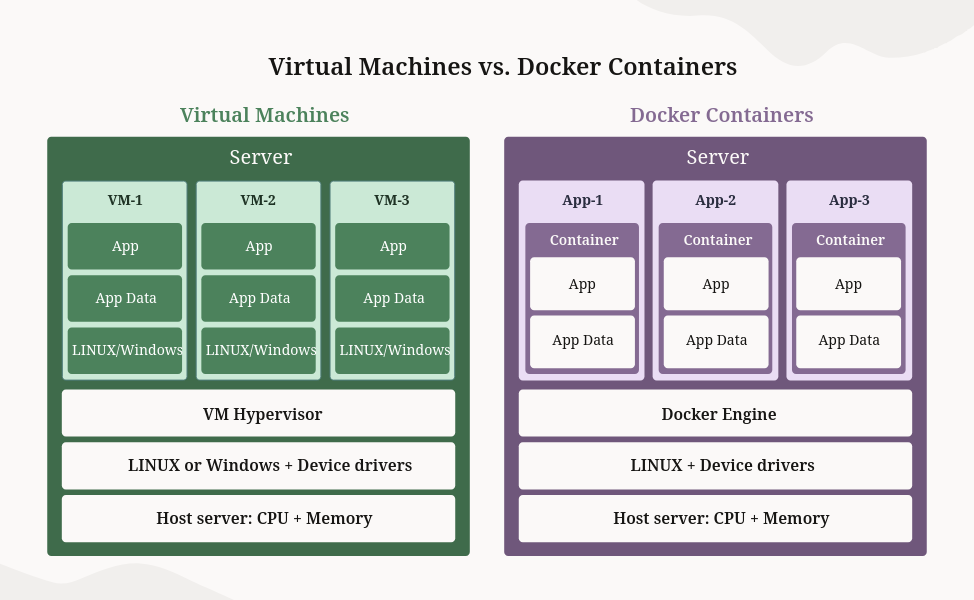
\includegraphics[width=0.5\linewidth]{vmvsdocker.png}
    \caption{Differenze tra le architetture delle macchine virtuali vs container docker\cite{oracle_docker}}
    \label{fig:placeholder}
\end{figure}


\newpage

\section{Metodologia - Architettura di Riferimento}

\subsection{Uso dei container DinD}
L'esigenza di simulare una rete di nodi in cui ognuno è indipendente senza avere un'infrastruttura hardware adatta ha portato a valutare i vantaggi dei container rispetto alle macchine virtuali per simulare una rete di nodi. I container sono più leggeri da usare rispetto alle macchine virtuali, in quanto non richiedoo di virtualizzare un intero sistema operativo. Inoltre è possibile usare i container come nodi su cui esegue Docker nel caso in cui questi siano container DinD (Docker in Docker).

Normalmente, creare un container Docker dentro Docker non sarebbe possibile perché l'applicazione ha bisogno di determinati permessi per eseguire che gli consentano di modificare i propri namespaces e cgroups. Per poterlo fare, sono stati creati i container DinD:

Docker-in-docker (DinD) è una tecnica che consente di eseguire un container Docker all'interno di un altro container Docker. DinD rende facile creare un ambiente isolato per ciascuna applicazione o servizio in fase di testing in una piattaforma CI\cite{dockercon2023_dind} (Continuos Integration, una pratica per cui diversi sviluppatori lavorano allo stesso codice modificandolo con merge frequenti in cui la CI fa verifica e testing automatizzato).\\\\
Sebbene sembrino perfetti allo scopo, lo stesso creatore della tecnica DinD (Petazzoni) mette in guardia dall'usare i container DinD nel campo delle piattaforme CI perché richiedono di dare a questi ultimi dei privilegi da amministratore (--privileged flag) che gli consentono di modificare i namespace e cgroups allo stesso livello del Docker che viene eseguito sull'host perdendo così l'isolamento dell'host. Hanno anche altri problemi come il non poter usare le stesse immagini presenti sul docker host, che richiede il dover cancellare la cache dei container DinD e scaricare nuovamente le immagini ad ogni build che impatta sui tempi di testing della build.\cite{petazzoni_dind}

Petazzoni consiglia invece di usare un'altra soluzione che ora viene definita come DooD (Docker outside of Docker), questa soluzione consiste nel condividere il socket UNIX di Docker dell'host (/var/run/docker.sock) con il container tramite un montaggio di volume (-v). In questo modo, il client Docker all'interno del container non esegue un proprio demone, ma invia le istruzioni direttamente al demone dell'host. Questo farà in modo che vengano creati container siblings e non figli di quel container, ma la cache sarà condivisa tra le diverse instanze risolvendo parte del problema\cite{petazzoni_dind}.

È stato comunque scelto di usare i container DinD, in quanto l'applicazione non verrà sviluppata su una pipeline CI in cui si susseguono molte modifiche con testing automatizzato e i container da usare saranno leggeri abbastanza da non subire problemi di perfomance a causa dei pull da fare durante il testing.
\subsection{Docker Swarm}
Dopo aver definito quali saranno i nodi che dovrà gestire l'orchestratore, analizziamo adesso Docker Swarm per avere un'architettura di riferimento su cui basare le funzionalità da implementare.

Docker include una Swarm mode per gesitre nativamente un cluster di Docker Enginges definito come uno "swarm". Permette di utilizzare l'interfaccia di Docker per creare uno swarm, fare deploy di servizi all'interno di uno swarm e di gestire il comportamento di quello swarm. \cite{docker_swarm}
\newpage
Uno "swarm" consiste di diversi Docker host che lo eseguono in Swarm mode, ciascun Docker host può essere un manager, un worker o entrambi: 
\begin{itemize}
    \item Manager, i nodi che agiscono da manager gestiscono la membership dei nodi e la delegazione di servizi.
    \item Worker, si occupano di eseguire i servizi delegati dai manager.
\end{itemize}

Un "servizio" in questo caso è una definizione dei task da eseguire sui nodi. Fa parte della struttura centrale di un sistema Swarm ed è il punto di interazione dell'utente con il sistema Swarm.\\
Alla creazione di un servizio, è possibile specificare il numero di repliche di quel servizio, quale container image usare, che risorse assegnare, la rete, e quali comandi eseguire all'interno dei container in esecuzione.\cite{docker_swarm_key_concepts}

Un "task" è un container in esecuzione, che fa parte di uno swarm service ed è gestito dai swarm manager.\\
Se vengono create più repliche di uno stesso servizio, uno Swarm manager distribuirà il numero di task repliche specificato tra i nodi nel modo che l'utente ha specificato come desired state.
Docker lavora per mantenere lo stato desiderato dall'utente, ad esempio se un worker node risulta inattivo allora Docker schedula i task di quel nodo su altri nodi worker.\cite{docker_swarm_key_concepts}

I passi seguiti per avviare un servizio quindi sono:
\begin{enumerate}
    \item l'utente crea un servizio e specifica all'orchestratore quante repliche avviarne 
    \item l'orchestratore si occupa di avviare dei task distribuendoli tra i nodi presenti
    \item  se durante l'esecuzione avviene un problema con un nodo allora l'orchestratore si occuperà di ridistribuire i task che stava eseguendo su altri nodi.
\end{enumerate}

\begin{figure}[H]
    \centering
    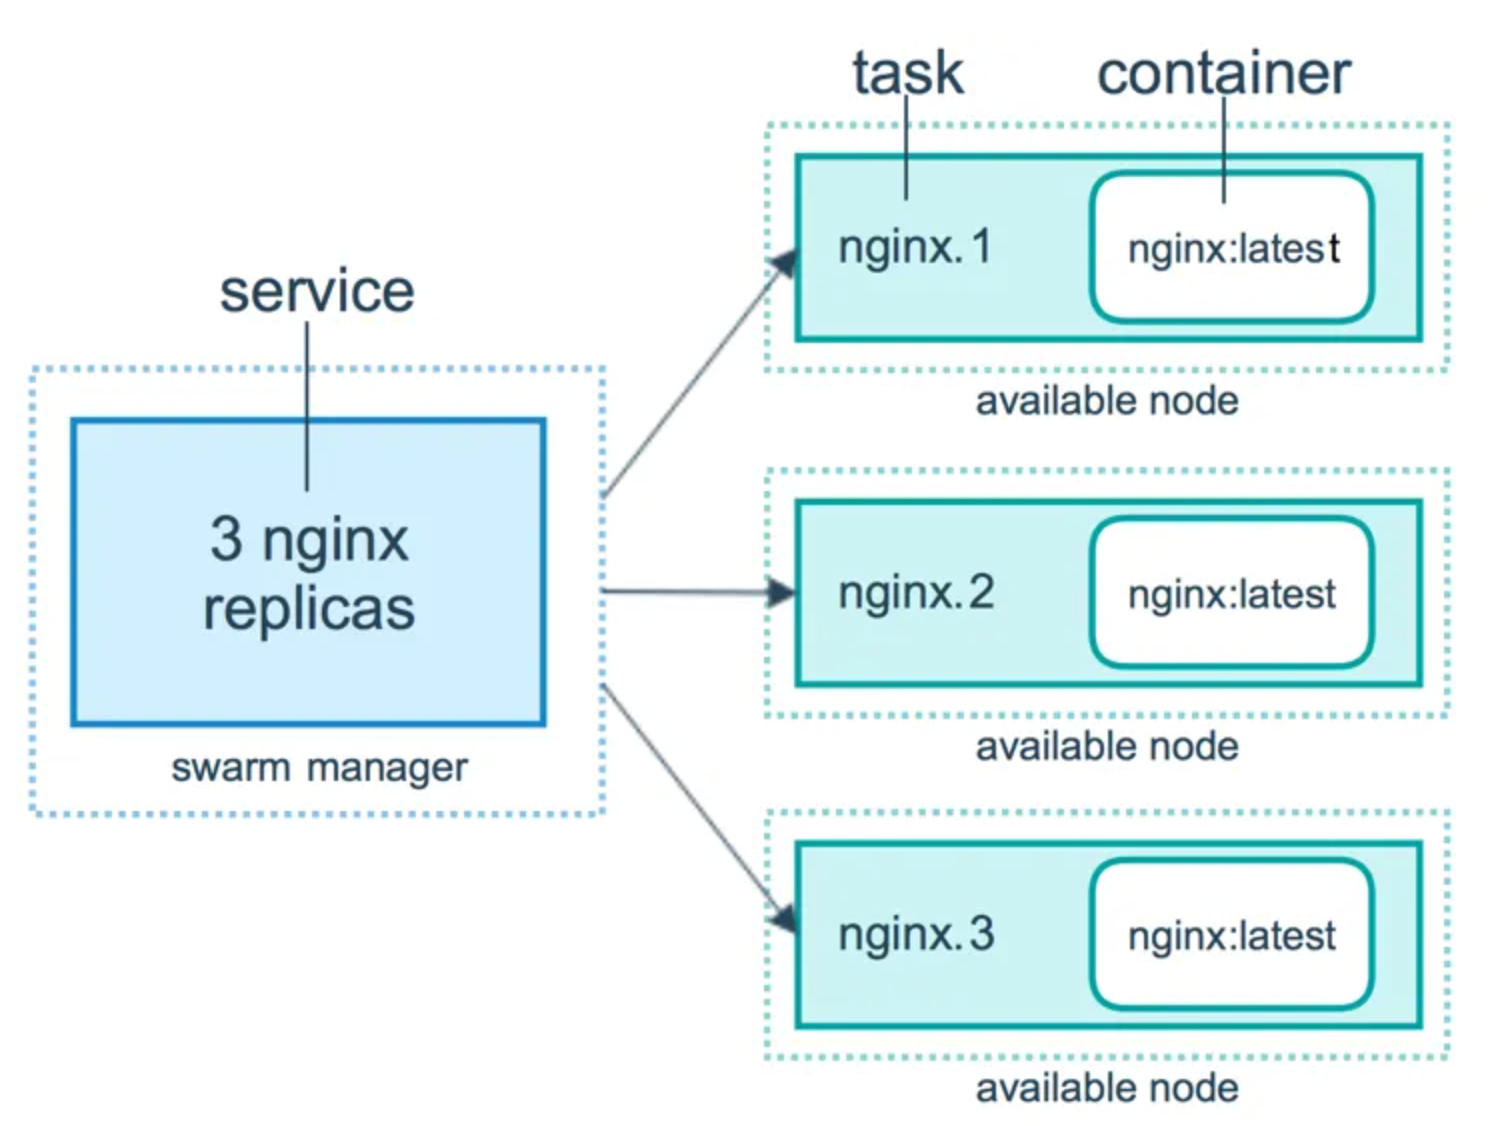
\includegraphics[width=0.8\linewidth]{image.png}
    \caption{Servizi, task e container in Docker Swarm \cite{immagine_servizi_swarm}}
    \label{fig:placeholder}
\end{figure}
\newpage
Le caratteristiche di Docker Swarm sono:
\begin{itemize}
    \item Design Decentralizzato, invece di gestire la differenziazione tra nodi durante il deployment, il Docker Engine permette di specializzare a runtime. È possibile costruire un inteor swarm tramite una singola disk image.
    \item Scaling, per ogni servizio è possibilie dichiarare il numero di task da eseguire. Quando avviene lo scale-up o scale-down (ovvero si aumenta o diminuisce il numero di repliche) lo Swarm Manager si adatta aggiungendo o rimuovendo i task per mantenere lo stato desiderato.
    \item Riconciliazione dello stato desiderato, lo Swarm Manager monitora costantemente lo stato del cluster e riconcilia le differenze tra lo stato attuale e quello espresso nello stato desiderato dall'utente. Ad esempio, se un servizio viene impostato per essere eseguito su 10 repliche e un worker che conteneva due di queste repliche diventa inattivo allora il manager crea due nuove repliche per rimpiazzare quelle che non sono più attive. Lo swarm manager assegnerà quelle repliche a dei nodi worker che sono ancora operativi e disponibili.
    \item Load Balancing, è possibile esporre le porte dei servizi a un load balancer esterno. Internamente swarm permette di specificare come distribuire i servizi dei container tra i nodi.
    \item Sicuro di default, ogni nodo di swarm usa una autenticazone mutual TLS e crittografia per comunicazioni sicure fra se stesso e gli altri nodi.\cite{docker_swarm}
\end{itemize}

Nella progettazione dell'orchestratore si terrà conto di queste caratteristiche per decidere quali funzionalità aggiungere.

\newpage

\section{Metodologia - Progettazione dell'Orchestratore}
\subsection{Ambiente dell'orchestratore}
Per simulare un sistema distribuito su cui l'orchestratore dovrà operare verranno usati i container DinD, ciascun container sarà un nodo worker e un ulteriore container contenente il codice dell'orchestratore sarà il nodo manager.

\begin{figure}[H]
    \centering
    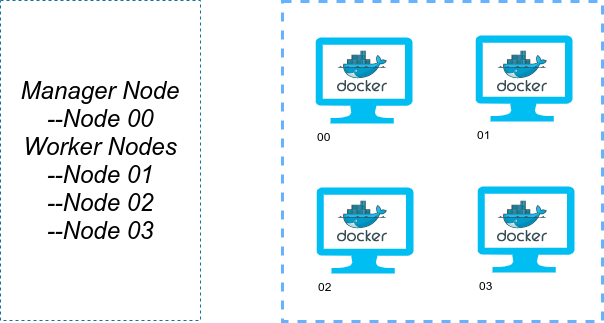
\includegraphics[width=0.5\linewidth]{docker_4_nodi.png}
    \caption{1 Nodo Manager e 3 Nodi Worker  \cite{supportlobby_swarm}}
    \label{fig:placeholder}
\end{figure}

\subsection{Comandi e operazioni di Docker Swarm}

Dato che l'architettura di riferimento è Docker Swarm, si osservano alcuni dei comandi utilizzabili tramite la CLI di Docker da poter implementare:

\begin{itemize}
    \item swarm init, inizializza lo swarm. Il Container Engine che viene selezionato per questo comando diventa il manager di una nuova rete swarm di cui è il singolo nodo.
    \item swarm join, fa unire un nodo ad uno swarm. In base alla --token flag passata il nodo entra nel swarm come manager o come worker. \cite{docker_swarm_cli}\\
    
    \item service create, crea un servizio con i parametri specificati. Il manager si occupa di farlo eseguire su uno dei nodi worker.
    \item service ps, stampa una lista dei task di un servizio che stanno attualmente eseguendo sul swarm.
    \item service rm, interrompe e rimuove i servizi specificati dal swarm.
    \item service scale, permette di scalare una o più repliche in un numero più basso o alto di repliche specificato. Il comando ritorna subito, ma ci vorrà del tempo per far avvenire lo scaling effettivo delle repliche. Se si vuole azzerare il numero di repliche esso si può scalare a 0. \cite{docker_service_cli}\\
    
    \item docker node ls, stampa una lista dei nodi che Docker Swarm conosce.
    \item docker node ps, stampa una lista di tutti i task su un nodo che Docker Swarm conosce. \cite{docker_node_cli}
    \newpage
    \item docker node update, permette di aggiornare i metadati di un nodo come la disponibilità, i suoi labels o il ruolo. \\In particolare, è possibile impostare la sua disponibilità come "Drain" (--avaiability drain), mentre il nodo è in questo stato lo scheduler non gli assegnerà altre task. Lo scheduler spegnerà eventuali task già esistenti sul nodo e le schudulerà su altri nodi disponibili. Questa modalità è utile nel caso in cui si voglia fare manutenzione sul nodo senza necessariamente spegnerlo o scollegarlo dalla rete.\cite{docker_manage_nodes}
\end{itemize}

\subsection{Fault Tolerance in Docker Swarm}
Per adempiere alle funzionalità di un orchestratore sarà necessario gestire anche i casi in cui i nodi falliscono o casi in cui i container facenti parte dei nodi si spengano occupando così spazio su disco (Garbage Collection).

Un sistema si definisce Fault Tolerant quando può tollerare un certo livello di fallimento, le fasi operative per gestire un guasto sono:
\begin{itemize}
    \item Failure Detection, si usano dei meccanismi di heartbeat per controllare se uno dei componenti del sistema sia fallito. Un segnale di heartbeat viene mandato periodicamente da un componente ad un altro dei componenti del sistema, se entro un certo tempo non ottiene risposta allora è stato riconosciuto un fallimento.
    \item System Reconfiguration/Mitigation, una volta riconosciuto il fallimento bisogna riconfigurare il sistema tramite dei meccanismi di Failover. Questi meccanismi di failover possono essere di Active-Passive Failover (se un componente attivo fallisce, uno in standby prende il suo posto) o di Active-Active Failover (più componenti sono già attivi, se uno fallisce il suo carico viene distribuito agli altri).
    \item Recovery, una volta mitigato il problema è necessario ristabilire il componente fallito. Ciò può avvenire tramite metodi come: Rollback Recovery (dopo aver identificato un errore il sistema ritorna ad uno stato precedente tramite checkpoints o i suoi logs), Forward Recovery (il sistema prova a correggere l'errore e continuare ad operare).\cite{tanenbaum_distributed_systems_4}
\end{itemize}

\begin{figure}[H]
    \centering
    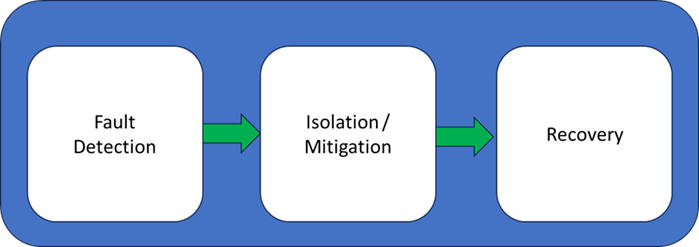
\includegraphics[width=0.8\linewidth]{fault_tolerance.png}
    \caption{Ciclo di Fault Tolerance di un Sistema \cite{mathworks_fdir}}
    \label{fig:placeholder}
\end{figure}

Docker Swarm gestisce la Fault Tolerance controllando lo stato desiderato di servizi dell'utente, nel caso in cui lo stato desiderato non corrisponda a quello attuale (ad esempio, un nodo è diventato inattivo e i suoi task non sono più in esecuzione) si occupa di distribuire il carico sugli altri nodi worker ancora in esecuzione.\cite{docker_how_services_work} Quindi un meccanismo di Active-Active Failover.

Nell'implementazione dell'orchestratore si terrà conto di queste funzionalità per aumentare la sua resilienza ai guasti.

\newpage
\subsection{Garbage Collection in Docker Swarm}
In Docker Swarm un task è l'unità atomica di esecuzione che progredisce in una successione definita di stati, dalla fase di assegnazione iniziale fino al suo completamento o fallimento. Nel caso di fallimento di un task l'orchestratore crea una nuova istanza di quel task, il task precedente non viene più utilizzato e quel container rimane spento e inutilizzato su quel nodo.\cite{docker_how_services_work}

Ciò vuol dire che gli oggetti non più utilizzati come container, immagini, volumi, reti e altri occuperanno spazio sul disco senza una reale funzione. Per eliminare questi oggetti esiste il comando "prune" da eseguire localmente sul nodo, che permette di eliminare determinati oggetti non più utilizzati su quel nodo.\cite{docker_pruning}

I task gestiti dall'orchestratore possono essere definiti come stateless, la loro esecuzione non dipende dallo stato interno di istanze precedenti. Se si scegliesse un approccio di tipo stateful il sistema proverebbe a preservare lo stato e il file system locale del container al riavvio di quest'ultimo, introducendo il rischio di avere stati corrotti dovuti al guasto del task precedente. Questo si traduce in un comportamento simile all'uso del comando "run" per la creazione di un task rispetto ad usare il comando "start" per riavviare un container già esisente.

Nell'implementazione dell'orchestratore si terrà conto di questa caratteristica, implementando un comportamento mirato al rilevamento e alla pulizia dei task falliti sui nodi per una gestione più efficiente della memoria sui nodi worker.
\newpage

\section{Implementazione}
\subsection{Struttura del sistema}
L'orchestratore è progettato per operare come nodo manager all'interno di un sistema distribuito, i nodi su cui verranno eseguiti i task saranno i nodi worker.\\
Questo sistema distribuito sarà simulato tramite Docker:
\begin{itemize}
    \item nodo manager, su cui verrà eseguito l'orchestratore con cui l'utente potrà interagire sarà un container con una immagine personalizzata di Python.
    \item nodi worker, saranno dei container con immagini docker:dind che seguiranno le istruzioni fornite dal nodo manager.
\end{itemize}

Per focalizzare lo sviluppo sulle funzionalità di esecuzione dei task sui nodi richiesto dalle specifiche del progetto, si è scelto di avere un ambiente composto da 1 nodo manager e 3 nodi worker.

\subsection{Linguaggi e Librerie Usate}
Per lo sviluppo dell'orchestratore è stato scelto Python 3, che permette facilmente di comunicare con il Docker Daemon dei vari nodi utilizzando la Docker API.

Le librerie usate sono:
\begin{itemize}
    \item docker (Docker SDK for Python): è la libreria ufficiale per interagire con il Docker Daemon in locale e in remoto. Consente di mandare istruzioni al Docker Daemon per gestire i container come il loro avvio, arresto, gestione delle reti, dei volumi, del loro stato e altro ancora.
    \item threading: per la gestione della concorrenza. Permette di eseguire in background il thread di monitoraggio (Failure Detection) che il thread dedicato alla gestione delle richieste dell'utente.
    \item queue: per implementare una coda thread-safe (FIFO) consentendo ai vari thread di accodare in modo sicuro i messaggi e le operazioni. Questo permette al thread principale di elaborare le azioni da eseguire sui nodi in modo sequenziale, evitando race condition.
    \item time: per la gestione dei controlli periodici sui nodi, oltre a rendere più facile per l'utente il tracciamento delle operazioni eseguite dall'orchestratore.
    \item uuid: per gestire identificativi univoci da associare ad ogni task creato sui nodi worker. Così da evitare conflitti di nomi tra container con nomi uguali all'interno dei nodi worker.
\end{itemize}

\subsection{Deploy}
Per inizializzare l'ambiente in cui l'orchestratore opera sono stati usati:
\begin{itemize}
    \item requirements.txt, contiene le librerie esterne necessarie per eseguire il codice dell'orchestratore.
    \item Dockerfile, usato per la costruzione dell'immagine Docker usata dall'orchestratore. I layer specificati la rendono un immagine Python 3.12, a cui vengono aggiunte le librerie esterne, copiato il codice dell'orchestratore e un comando per eseguirlo all'avvio del container.
    \item docker-compose.yaml, un file che inizializza il nodo manager con l'immagine del Dockerfile, 3 nodi worker con immagine docker:dind e connette tutti i nodi sulla stessa network.
\end{itemize}
\newpage
\subsection{Strutture Dati}
\begin{center}
\textbf{nodo.py}
\end{center}
\begin{minted}{Python}
class Nodo:
    def __init__(self, nome, ip, timeout=3):
        self.nome = nome
        self.ip = ip
        self.timeout = timeout
        try:
            self.client = docker.DockerClient(base_url=f'tcp://{ip}:2375', timeout=self.timeout)
        except DockerException:
            print(f"Info> Attenzione: impossibile connettersi a {nome} ({ip}) alla creazione. Verrà considerato down finché non risponde.")
            self.client = None
        self.container_attivi = {}
        self.disponibile = True
\end{minted}
Questa classe è usata per definire una connessione con un nodo worker e gestire il suo stato durante l'esecuzione. L'attributo "ip" viene utilizzato per connettersi con il container DinD (ovvero un nodo worker), una volta stabilita la connessione viene creato un oggetto DockerClient con cui è possibile dare ordini al Docker Eninge del nodo worker.\\
Tramite l'attributo "container\_attivi" tiene traccia dei task attivi sul nodo e l'attributo "disponibile" permette agli altri componenti di sapere se il nodo può accettare nuove task o se è in stato di Drain.

I suoi metodi consentono di visualizzare le informazioni riguardo ai container attivi e spenti sul nodo.
\begin{center}
\textbf{config.py}
\end{center}
\begin{minted}{Python}
class Config:
    def __init__(self, image, servizio_name, command=None):
        self.image = image
        self.command = command
        self.servizio_name = servizio_name
\end{minted}
Questa classe è usata per tenere traccia dei servizi definiti. Per ciascun servizio assegna un nome (che sarà anche nel nome della task al suo avvio), un immagine e opzionalmente un comando da eseguire. 
\begin{center}
\textbf{menu.py}
\end{center}
\begin{minted}{Python}
class Menu:
    def __init__(self, lista_nodi, coda, servizi_validi):
        self.lista_nodi = lista_nodi
        self.coda = coda
        self.servizi = servizi_validi
\end{minted}
Questa classe è usata per permettere all'utente di interagire con l'orchestratore. Contiene gli attributi necessari per mandare richieste al thread manager.\\
I suoi metodi sono relativi all'interazione con l'utente come creare nuovi task di un servizio, gestire lo stato dei nodi e mandare richieste al thread manager quando necessario.
\subsection{Gestione dei Nodi}
\begin{center}
\textbf{main.py}
\end{center}
\begin{minted}{Python}
lista_nodi = {
    "nodo1": Nodo("nodo1", "nodo1avo"),
    "nodo2": Nodo("nodo2", "nodo2avo"),
    "nodo3": Nodo("nodo3", "nodo3avo"),
}

servizi_validi = [
    Config("alpine", servizio_name="alpine.sleep", command="sleep infinity"),
    Config(image="hello-world", servizio_name="basic.hello.world"),
]
\end{minted}
Eseguendo l'orchestratore vengono viene inizializzato un dizionario contenente le istanze dei nodi presenti nell'infrastruttura. In questo caso l'indirizzo (hostname) dei nodi corrisponde al nome del loro container DinD, questo è possibile grazie al servizio DNS che il Docker Engine usa per la risoluzione automatica dei nomi tra container che fanno parte della stessa rete.

Viene anche creata una lista dei servizi di default che l'utente può usare all'avvio dell'orchestratore. Sono state scelte delle container image leggere per mostrare le funzionalità dell'orchestratore senza appesantire la macchina host.

Infine si occupa di avviare il thread manager e il thread failure\_detection, condividendo con loro la lista dei nodi e la coda delle richieste.
\begin{center}
\textbf{cluster.py}
\end{center}
\begin{minted}{Python}
def deploy_container(nodo, config):
    try:
        nodo.client.containers.run(**config)
        print(f"\nInfo> Task: {config['image']} deployato (run) sul nodo: {nodo.nome}")
    except Exception as e:
        print("Errore nel deploy del task: ", e)

\end{minted}
Questo file contiene le funzionalità in cui viene usata la Docker API tramite i DockerClient di ciascun nodo e altre funzionalità per la gestione del cluster. Queste sono:
\begin{itemize}
    \item deploy\_container, fa partire una task sul nodo specificato.
    \item stop\_container, ferma una task che sta venendo eseguita sul nodo specificato.
    \item remove\_container, rimuove una task spenta sul nodo specificato.
    \item disponibilita\_nodi, controlla la disponibilità dei nodi ritornando una lista dei nomi dei nodi attivi.
    \item list\_nodes, usata per ottenere informazioni sui task attualmente attivi sui nodi e il loro stato. Ritorna un dizionario con le liste di tutti i task che stanno eseguendo su tutti i nodi della rete.
\end{itemize}
\subsection{Thread: Manager}
\begin{center}
\textbf{main.py}
\end{center}
\begin{minted}{Python}
    coda = queue.Queue()

    thread_manager = threading.Thread(target=manager, args=(lista_nodi, coda), daemon=True)

    thread_manager.start()
\end{minted}
All'esecuzione del codice viene inizializzato l'oggetto Queue, che permette di creare una coda FIFO thread-safe basata su meccanismi di mutua esclusione. Questa coda funge da canale asincrono in cui aggiungere richieste che il thread manager preleva ed elabora sequenzialmente.
\begin{center}
\textbf{manager.py}
\end{center}
\begin{minted}{Python}
def manager(lista_nodi, coda):
    while True:
        try:
            richiesta = coda.get(timeout=1)
            
            try:
                print(f"\nManager> Schedulo ", richiesta["azione"], ' ', end="")
                if isinstance(richiesta["target"], Config):
                    print(" ==> ", end='')
                    richiesta["target"].stampa_config()
                attiva_nodo
                azione = richiesta["azione"]
                target = richiesta["target"]
                
                match azione:
                    case "deploy":
                        schedula_servizio(target, lista_nodi, list_nodes(lista_nodi))
                    case "scale_down":
                        spegni_servizio(target, lista_nodi, list_nodes(lista_nodi))
                    case "drain_nodo":
                        disattiva_svuota_nodo(target, lista_nodi, coda)
                    case "attiva_nodo":
                        attiva_nodo(target, lista_nodi)
                    case _:
                        print(f"Manager> Azione sconosciuta: {azione}")
                
                list_nodes(lista_nodi, stampa=True)
            except Exception as e:
                print(f"Manager> Errore nella gestione della richiesta: {e}")
                
            finally:
                coda.task_done()
            rimuovi_container_spenti_tutti_nodi(lista_nodi)
            pass
            
        time.sleep(1)
\end{minted}
Il thread manager si occupa di prelevare richieste dalla coda e di eseguirle. I tipi di richiesta che gestisce sono:
\begin{itemize}
    \item deploy, quando il manager esegue un deploy avvia schedula\_servizio() passando come argomenti l'oggetto Config del servizio da avviare, la lista dei nodi e le statistiche attuali sui task che stanno eseguendo sui nodi in questo momento. A questo punto, schedula\_servizio() genera un nome univoco per il container e cerca nella lista di nodi quello con meno task attivi tramite la funzione trova\_nodo\_least\_loaded(), infine avvia la task sul nodo scelto con deploy\_container().
    \begin{minted}{Python}
def trova_nodo_least_loaded(lista_nodi, nodi_e_container):
    punteggi = {}
    for nodo, containers in nodi_e_container.items():
        if lista_nodi[nodo].disponibile:
            punteggio = len(containers)
            punteggi[nodo] = punteggio
    if not punteggi:
        return None
    return min(punteggi, key=lambda punteggio_nodo: punteggi[punteggio_nodo])
\end{minted}
    Questa funzione aggiunge una funzionalità essenziale di load balancing all'orchestratore. Prima di avviare un task, questa funzione cerca nel cluster il nodo con meno task attivi così da non sovraccaricare nodi che hanno già molti task attive su di essi e garantendo un bilanciamento dinamico durante l'esecuzione dei task.
    
    \item scale\_down, ferma un task del servizio specificato sul nodo del cluster che ha quel tipo di task attiva e ha più task attive in quel momento. Viene riconosciuto il nodo con più task attive tramite la funzione "trova\_nodo\_most\_loaded" e fermato il servizio su quel nodo.
    
    \item drain\_nodo, disattiva il nodo selezionato impostato come in Drain e manda richieste alla coda del manager per schedulare le task sugli altri nodi ancora disponibili. Quando in stato di Drain, un nodo non viene considerato quando avviene il deploy di un task.
    \begin{minted}{Python}
def disattiva_svuota_nodo(nome_nodo, lista_nodi, coda):
    nodo = lista_nodi[nome_nodo]
    nodo.disponibile = False
    lista_nodi_stats = list_nodes(lista_nodi)
    containers_da_spostare = lista_nodi_stats.get(nome_nodo, [])
    for container in containers_da_spostare:
        servizio_name = container["nome"].split("-")[0]
        config_ricreata = Config(
            image=container["immagine"],
            servizio_name=servizio_name,
            command=container.get("comando")
        )
        invia_richiesta(coda, "deploy", config_ricreata)
        stop_container(nodo, container["id"])
    print(f"\nManager> Nodo {nome_nodo} svuotato: {len(containers_da_spostare)} task rischedulati altrove.")
    \end{minted}
    \item attiva\_nodo, riattiva un nodo in stato di Drain. Da questo momento in poi il nodo potrà tornare ad essere considerato per il deploy di task.
\end{itemize}


Nel caso in cui non ci siano richieste da gestire, si occupa della garbage collection tramite la funzione "rimuovi-container\_spenti\_tutti\_nodi()" che controlla se ci sono task spenti sui nodi e se ci sono li rimuove in quanto non verranno usati di nuovo dall'orchestratore.
\subsection{Thread: Failure Detection}
\begin{center}
\textbf{main.py}
\end{center}
\begin{minted}{Python}
    thread_failure_detection = threading.Thread(target=failure_detection.heartbeat, args=(lista_nodi, coda, 5), daemon=True)
    thread_failure_detection.start()
\end{minted}
All'inizio dell'esecuzione, dopo il thread manager viene avviato il thread failure\_detection, che si occupa di controllare periodicamente lo stato di nodi e spostare i loro task sui nodi attivi nel caso uno di loro fallisca.
\begin{center}
\textbf{failure\_detection.py}
\end{center}
\begin{minted}{Python}
def heartbeat(lista_nodi, coda, intervallo=3):
    while True:
        try:
            for nome, nodo in lista_nodi.items():
                stato_nodo = nodo.is_up()
                if stato_nodo == False:
                    failover(nodo.container_attivi, nodo.nome, coda)
        except Exception as e:
            print(f"Failure_detection> Errore nel thread heartbeat: {e}")
        time.sleep(intervallo)    
\end{minted}
Questo thread si occupa di controllare lo stato dei nodi periodicamente, tramite heartbeat() controlla ogni "intervallo" secondi la lista dei nodi per vedere se sono ancora attivi. Se rileva che un nodo è diventato inattivo allora questo da inizio al meccanismo di failover. Questo aggiunge all'orchestratore una funzionalità di failure detection.
\begin{minted}{Python}
def failover(container_attivi_nodo, nome, coda):
    container_attivi = list(container_attivi_nodo)
    container_attivi_nodo.clear()
    if len(container_attivi) == 0:
        return
    for container in container_attivi:
        servizio_name = container["nome"].split("-")[0]
        config_ricreata = Config(
            image=container["immagine"],
            servizio_name=servizio_name,
            command=container["comando"])
        invia_richiesta(coda, "deploy", config_ricreata)
    print(f"\nFailure_detection> Il nodo {nome} aveva questi task attivi e verranno rischedulati: {container_attivi}")
\end{minted}
Tramite failover() si ottengono i task presenti sul nodo quando era ancora attivo, questi vengono poi schedulati tramite richieste al manager che li avvierà nel modo corretto sui nodi attivi rimasti. L'orchestratore può quindi fare una system reconfiguration che permette al sistema di continuare ad eseguire task anche nel caso di un eventuale guasto di un nodo.
\newpage
\subsection{Interfaccia Utente}
\begin{center}
\textbf{main.py}
\end{center}
\begin{minted}{Python}
    menu = Menu(lista_nodi, coda, servizi_validi)
    menu.avvia_menu()
\end{minted}
All'avvio del programma, dopo aver avviato i due thread precedenti, viene istanziato un oggetto Menu e poi avviato tramite un suo metodo per mostrare l'interfaccia all'utente.
\begin{center}
\textbf{menu.py}
\end{center}
Il menù mostrato all'utente si compone di tre schermate:
\begin{itemize}
    \item avvia\_menu(), da cui è possibile accedere alle altre due schermate, aggiungere alla lista servizi\_disponibili la configurazione di un servizio personalizzabile dall'utente e uscire dal programma.
    \item menu\_servizi(), da cui è possibile scegliere di creare una replica di un servizio a scelta dell'utente fra la lista servizi\_disponibili oppure scalare (aumentare, diminuire, azzerare) il numero di repliche di un servizio scelto dall'utente.
    \item menu\_stato\_nodi(), da cui è possibile monitorare lo stato attuale dei nodi e i task eseguiti attualemente su ciascun nodo. Inoltre è possibile impostare un nodo in stato Drain o riattivarlo.
\end{itemize}
Le scelte dell'utente che riguardano i task o il cambio di stato di un nodo causano l'aggiunta di una o più richieste nella coda del thread manager, così che vengano eseguite sequenzialmente quando arriverà il loro turno nella coda.

A supporto dell'interfaccia, la classe usa altri metodi che si occupano: del conteggio delle repliche attive e tradurre le opzioni selezionate in una sequenza di richieste che verranno inoltrate alla coda per l'elaborazione da parte del thread manager.
\begin{center}
\textbf{utils.py}
\end{center}
\begin{minted}{Python}
def scegli_config():
    immagine = input("Che immagine vuoi usare? Scrivi il nome di un immagine esistente di cui ogni nodo potrà fare il pull\n")
    servizio_name = input("Che nome vuoi dare a questo servizio custom? ...")
    if "-" in servizio_name:
        return None
    comando = input("Che comando vuoi usare sul container? Lascia vuoto per nessun comando\n")
    return Config(immagine, servizio_name, command=comando)
\end{minted}
Il modulo utils.py raccoglie funzioni che forniscono operazioni di supporto al resto del sistema. Tra queste ci sono:
\begin{itemize}
    \item scegli\_config(), che permette all'utente di dare un nome ad un servizio e scegliere per quest'ultimo un immagine e un comando da eseguire.
    \item is\_container\_vecchio(), che serve per verificare se un task all'interno di un nodo è in stato di "created" da troppo tempo e quindi non si avvierà. Questo può succedere nel momento in cui un nodo non riesce ad avviare una task perché un comando non è adatto a quella container image o altri motivi.
\end{itemize}
\newpage

\section{Risultati}
\subsection{Deploy e Scaling dei Servizi}
La prima voce del menù permette di avviare una singola istanza di un servizio, questa verrà schedulata sul nodo meno carico del cluster:
\begin{minted}{text}
---Menu Servizi---
Scegli una voce dal menù:
1) Crea replica di 1 servizio
2) Scala N repliche di un servizio
3) Torna al Menu Principale
1
Scegli quale servizio avviare tra quelli disponibili:
1) Immagine: alpine | Nome Servizio: alpine.sleep | Comando: sleep infinity
2) Immagine: hello-world | Nome Servizio: basic.hello.world
1
Manager> Schedulo  deploy   ==> Immagine: alpine | Nome Servizio: alpine.sleep | Comando: sleep infinity
Info> Task: alpine deployato (run) sul nodo: nodo1
nodo1 | UP | Task attivi(1): 
nome : alpine.sleep-9c050d42b7 | id : 0a0d9d183285 | immagine : alpine:latest | comando : sleep infinity | 
nodo2 | UP | Task attivi(0): 
nodo3 | UP | Task attivi(0): 
\end{minted}
La seconda voce del menù permette di avviare una operazione di scaling, così che l'utente possa impostare il numero desiderato di repliche per un servizio e il sistema possa ricalibrare il numero di task in base alla scelta dell'utente:
\begin{minted}{text}
---Menu Servizi---
Scegli una voce dal menù:
1) Crea replica di 1 servizio
2) Scala N repliche di un servizio
3) Torna al Menu Principale
2
Scegli quale servizio vuoi scalare
1) Immagine: alpine | Nome Servizio: alpine.sleep | Comando: sleep infinity
2) Immagine: hello-world | Nome Servizio: basic.hello.world
1
Scegli il numero di repliche che vuoi avere per il servizio scelto
4
nodo1 | UP | Task attivi(2): 
nome : alpine.sleep-c468f0e906 | id : 6197bda48875 | immagine : alpine:latest | comando : sleep infinity | 
nome : alpine.sleep-9c050d42b7 | id : 0a0d9d183285 | immagine : alpine:latest | comando : sleep infinity | 
nodo2 | UP | Task attivi(1): 
nome : alpine.sleep-0e9073b0fe | id : ae962553a84b | immagine : alpine:latest | comando : sleep infinity | 
nodo3 | UP | Task attivi(1): 
nome : alpine.sleep-ea97c1f21d | id : fbd19afd6887 | immagine : alpine:latest | comando : sleep infinity | 
\end{minted}
\newpage
La seconda voce del menù permette anche lo scale down di un servizio, durante questo processo vengono scelti i nodi che hanno quel servizio con più task attivi in quel momento e se possibile si tolgono più task da quel nodo:
\begin{minted}{text}
---Menu Servizi---
Scegli una voce dal menù:
1) Crea replica di 1 servizio
2) Scala N repliche di un servizio
3) Torna al Menu Principale
2
Scegli quale servizio vuoi scalare
1) Immagine: alpine | Nome Servizio: alpine.sleep | Comando: sleep infinity
2) Immagine: hello-world | Nome Servizio: basic.hello.world
1
Scegli il numero di repliche che vuoi avere per il servizio scelto
2
(...)
nodo1 | UP | Task attivi(0): 
nodo2 | UP | Task attivi(1): 
nome : alpine.sleep-0e9073b0fe | id : ae962553a84b | immagine : alpine:latest | comando : sleep infinity | 
nodo3 | UP | Task attivi(1): 
nome : alpine.sleep-ea97c1f21d | id : fbd19afd6887 | immagine : alpine:latest | comando : sleep infinity | 
\end{minted}
Infine, la seconda voce permette anche di azzerare le repliche di un servizio:
\begin{minted}{text}
---Menu Servizi---
Scegli una voce dal menù:
1) Crea replica di 1 servizio
2) Scala N repliche di un servizio
3) Torna al Menu Principale
Manager> Task già spenti rimossi su nodo1: ['alpine.sleep-c468f0e906, alpine:latest', 'alpine.sleep-9c050d42b7, alpine:latest']
2
Scegli quale servizio vuoi scalare
1) Immagine: alpine | Nome Servizio: alpine.sleep | Comando: sleep infinity
2) Immagine: hello-world | Nome Servizio: basic.hello.world
1
Scegli il numero di repliche che vuoi avere per il servizio scelto
0
Richieste 2 rimozioni di repliche di 'alpine.sleep'
Manager> Schedulo  scale_down   ==> Immagine: alpine | Nome Servizio: alpine.sleep | Comando: sleep infinity
Info> Un task sul nodo nodo2 è stato fermato
Manager> Schedulo  scale_down   ==> Immagine: alpine | Nome Servizio: alpine.sleep | Comando: sleep infinity
Info> Un task sul nodo nodo3 è stato fermato
nodo1 | UP | Task attivi(0): 
nodo2 | UP | Task attivi(0): 
nodo3 | UP | Task attivi(0): 
\end{minted}
\newpage
\subsection{Stato dei nodi e dei Task}
Tramite le prime due voci del Menù Stato Nodi è possibile visualizzare lo stato dei nodi e i task in esecuzione (o terminati) su ciascun nodo del cluster: 
\begin{minted}{text}
---Menu Stato Nodi---
Scegli una voce dal menù:
1) Stampa stato e task attivi sui nodi
2) Stampa stato e task attivi e spenti sui nodi
3) Svuota un nodo 
4) Attiva un nodo se è in DRAIN 
5) Torna al Menu Principale
1
nodo1 | UP | Task attivi(1): 
nome : alpine.sleep-7a2ee9f608 | id : 5d5909aed749 | immagine : alpine:latest | comando : sleep infinity | 
nodo2 | UP | Task attivi(0): 
nodo3 | UP | Task attivi(0): 
\end{minted}
\subsection{Creazione di Nuovi Servizi}
Con la terza voce del menù principale è possibile creare una nuova configurazione per un servizio, definendo il nome, l'immagine e il comando di esecuzione:
\begin{minted}{text}
---Menu Principale---
Scegli il numero di una voce dal menu:
1) Menu - Servizi
2) Menu - Stato Nodi
3) Aggiungi Configurazione Servizio
4) Uscita
5) Uscita Forzata (senza finire di gestire le richieste in coda)
3
Che immagine vuoi usare? Scrivi il nome di un immagine esistente di cui ogni nodo potrà fare il pull
busybox
Che nome vuoi dare a questo servizio custom? (Non usare nomi con il trattino '-')
busyboxsleep
Che comando vuoi usare sul container? Lascia vuoto per nessun comando
sleep infinity
---Menu Servizi---
Scegli una voce dal menù:
1) Crea replica di 1 servizio
(...)
1
Scegli quale servizio avviare tra quelli disponibili:
1) Immagine: alpine | Nome Servizio: alpine.sleep | Comando: sleep infinity
2) Immagine: hello-world | Nome Servizio: basic.hello.world
3) Immagine: busybox | Nome Servizio: busyboxsleep | Comando: sleep infinity
3
(...)
nodo2 | UP | Task attivi(1): 
nome : busyboxsleep-5ee4effa6f | id : 07ac0ad6fde8 | immagine : busybox:latest | comando : sleep infinity | 
\end{minted}
\newpage
\subsection{Nodi in stato di Drain}
Tramite la terza voce del Menù Stato Nodi è possibile svuotare un nodo mettendolo in Drain e facendo passare i suoi task in esecuzione su altri nodi:
\begin{minted}{text}
---Menu Stato Nodi---
Scegli una voce dal menù:
1) Stampa stato e task attivi sui nodi
2) Stampa stato e task attivi e spenti sui nodi
3) Svuota un nodo 
4) Attiva un nodo se è in DRAIN 
5) Torna al Menu Principale
3
Scegli quale nodo vuoi svuotare (andrà in stato di DRAIN)
1) nodo1
2) nodo2
3) nodo3
3
Manager> Schedulo  drain_nodo
Manager> Nodo nodo3 svuotato: 1 task rischedulati altrove.
nodo1 | UP | Task attivi(2): 
nome : alpine.sleep-3ea3bf8e09 | id : 1d9a09c5a8e9 | immagine : alpine:latest | comando : sleep infinity | 
nome : alpine.sleep-7a2ee9f608 | id : 5d5909aed749 | immagine : alpine:latest | comando : sleep infinity | 
nodo2 | UP | Task attivi(2): 
nome : alpine.sleep-17e1ac63be | id : a06a19e76217 | immagine : alpine:latest | comando : sleep infinity | 
nome : busyboxsleep-5ee4effa6f | id : 07ac0ad6fde8 | immagine : busybox:latest | comando : sleep infinity | 
nodo3 | UP | Task attivi(0):
(...)
Nodi in stato di DRAIN: nodo3
\end{minted}
Mentre un nodo è in Drain non verrà considerato nell'assegnazione di nuovi task, restando vuoto fino a che non viene riattivato:
\begin{minted}{text}
---Menu Servizi---
Scegli una voce dal menù:
1) Crea replica di 1 servizio
2) Scala N repliche di un servizio
3) Torna al Menu Principale
1
Scegli quale servizio avviare tra quelli disponibili:
1) Immagine: alpine | Nome Servizio: alpine.sleep | Comando: sleep infinity
2) Immagine: hello-world | Nome Servizio: basic.hello.world
3) Immagine: busybox | Nome Servizio: busyboxsleep | Comando: sleep infinity
1
Manager> Schedulo  deploy   ==> Immagine: alpine | Nome Servizio: alpine.sleep | Comando: sleep infinity
Info> Task: alpine deployato (run) sul nodo: nodo2
nodo1 | UP | Task attivi(3): 
nome : alpine.sleep-02ed572f73 | id : 578e6d5015ed | immagine : alpine:latest | comando : sleep infinity | 
nome : alpine.sleep-3ea3bf8e09 | id : 1d9a09c5a8e9 | immagine : alpine:latest | comando : sleep infinity | 
nome : alpine.sleep-7a2ee9f608 | id : 5d5909aed749 | immagine : alpine:latest | comando : sleep infinity | 
nodo2 | UP | Task attivi(3): 
nome : alpine.sleep-5e1ebb77c6 | id : e4e7aaa48bb2 | immagine : alpine:latest | comando : sleep infinity | 
nome : alpine.sleep-17e1ac63be | id : a06a19e76217 | immagine : alpine:latest | comando : sleep infinity | 
nome : busyboxsleep-5ee4effa6f | id : 07ac0ad6fde8 | immagine : busybox:latest | comando : sleep infinity | 
nodo3 | UP | Task attivi(0): 
\end{minted}
Riattivazione del nodo:
\begin{minted}{text}
---Menu Stato Nodi---
Scegli una voce dal menù:
1) Stampa stato e task attivi sui nodi
2) Stampa stato e task attivi e spenti sui nodi
3) Svuota un nodo 
4) Attiva un nodo se è in DRAIN 
5) Torna al Menu Principale
4
Scegli quale nodo vuoi attivare (sarà di nuovo considerato per il deploy)
1) nodo3
1
Manager> Schedulo  attiva_nodo  
Manager> Nodo nodo3 attivato, torna a poter ricevere nuovi task.
\end{minted}
Adesso il nodo viene di nuovo considerato nell'assegnazione di nuove task:
\begin{minted}{text}
---Menu Servizi---
Scegli una voce dal menù:
1) Crea replica di 1 servizio
2) Scala N repliche di un servizio
3) Torna al Menu Principale
1
Scegli quale servizio avviare tra quelli disponibili:
1) Immagine: alpine | Nome Servizio: alpine.sleep | Comando: sleep infinity
2) Immagine: hello-world | Nome Servizio: basic.hello.world
3) Immagine: busybox | Nome Servizio: busyboxsleep | Comando: sleep infinity
1
Manager> Schedulo  deploy   ==> Immagine: alpine | Nome Servizio: alpine.sleep | Comando: sleep infinity
Info> Task: alpine deployato (run) sul nodo: nodo3
nodo1 | UP | Task attivi(3): 
(...)
nodo2 | UP | Task attivi(3): 
nome : alpine.sleep-5e1ebb77c6 | id : e4e7aaa48bb2 | immagine : alpine:latest | comando : sleep infinity (...)
nodo3 | UP | Task attivi(1): 
nome : alpine.sleep-664aef4b49 | id : 8720442c9a35 | immagine : alpine:latest | comando : sleep infinity | 
\end{minted}
\newpage
\subsection{Caduta di un nodo}
Per simulare la caduta di un nodo è possibile usare il comando "kilL" sul container DinD, il thread failure\_detection percepirà la caduta del nodo e reagirà:
\begin{minted}{Bash}
docker kill nodo1
\end{minted}
Questo era lo stato dei task prima della caduta del nodo:
\begin{minted}{text}
nodo1 | UP | Task attivi(3): 
(nome : alpine.sleep-02ed572f73 | id : 578e6d5015ed | immagine : alpine:latest | comando : sleep infinity | 
nome : alpine.sleep-3ea3bf8e09 | id : 1d9a09c5a8e9 | immagine : alpine:latest | comando : sleep infinity | 
nome : alpine.sleep-7a2ee9f608 | id : 5d5909aed749 | immagine : alpine:latest | comando : sleep infinity | )
nodo2 | UP | Task attivi(3): 
(...)
nodo3 | UP | Task attivi(1): 
(...)
\end{minted}
Dopo la caduta del nodo si è attivato il meccanismo di failover, che ha mandato in coda i task del nodo1 per poterli eseguire sui nodi attivi:
\begin{minted}{text}
Failure_detection> Il nodo nodo1 aveva questi task attivi e verranno rischedulati: [{'nome': 'alpine.sleep-02ed572f73', 'id': '578e6d5015ed', 'immagine': 'alpine:latest', 'comando': 'sleep infinity'}, {'nome': 'alpine.sleep-3ea3bf8e09', 'id': '1d9a09c5a8e9', 'immagine': 'alpine:latest', 'comando': 'sleep infinity'}, {'nome': 'alpine.sleep-7a2ee9f608', 'id': '5d5909aed749', 'immagine': 'alpine:latest', 'comando': 'sleep infinity'}]
Manager> Schedulo  deploy   ==> Immagine: alpine:latest | Nome Servizio: alpine.sleep | Comando: sleep infinity
nodo1 | DOWN
Info> Task: alpine:latest deployato (run) sul nodo: nodo3
(...)
nodo1 | DOWN
nodo2 | UP | Task attivi(4): 
nome : alpine.sleep-bc5a25cc9f | id : 81d24b5c15c3 | immagine : alpine:latest | comando : sleep infinity | 
nome : alpine.sleep-5e1ebb77c6 | id : e4e7aaa48bb2 | immagine : alpine:latest | comando : sleep infinity | 
nome : alpine.sleep-17e1ac63be | id : a06a19e76217 | immagine : alpine:latest | comando : sleep infinity | 
nome : busyboxsleep-5ee4effa6f | id : 07ac0ad6fde8 | immagine : busybox:latest | comando : sleep infinity | 
nodo3 | UP | Task attivi(3): 
nome : alpine.sleep-93a6d06d5b | id : 260e603e7a3a | immagine : alpine:latest | comando : sleep infinity | 
nome : alpine.sleep-5021a0c20f | id : b9206207e4c0 | immagine : alpine:latest | comando : sleep infinity | 
nome : alpine.sleep-664aef4b49 | id : 8720442c9a35 | immagine : alpine:latest | comando : sleep infinity | 

\end{minted}
\newpage

\section{Limiti e Sviluppi Futuri}
Nonostante le funzionalità implementate, il sistema presenta alcuni limiti architetturali che potrebbero essere risolti con futuri miglioramenti.

Alcuni di questi limiti sono:
\begin{itemize}
    \item Attualmente non è possibile eliminare voci dalla lista dei servizi disponibili o modificarli.
    \item La garbage collection si limita a ripulire i task spenti sul nodo, questo potrebbe essere esteso ad eliminare anche immagini, network e altri oggetti inutilizzati. Inoltre il fatto che i task spenti vengano eliminati in modo automatico non permette un'analisi approfondita sul fallimento del task, che aiuterebbe a non far ripresentare il problema ulteriormente.
    \item In questo momento i task consentono di specificare soltanto l'immagine e un comando da eseguire su di essa, è possibile espandere questa funzionalità includendo le limitazioni dell'uso della CPU, memoria disponibile per il task e le altre già disponibili grazie al Docker Engine.
    \item Ci sono dei limiti di sicurezza rappresentati dal fatto che i container DinD hanno bisogno di avere il flag "--privileged" attivo, il che fa perdere al docker host l'isolamento dai nodi stessi.
\end{itemize}

In futuro si potrebbe evolvere l'orchestratore per una gestione del sistema distribuito più simile a Docker Swarm con:
\begin{itemize}
    \item Per lo scopo del progetto si è scelto di avere un ambiente contenuto con un numero statico di nodi, ma sarebbe possibile espandere questa funzionalità permettendo ad altri nodi di unirsi durante l'esecuzione previa richiesta al nodo manager. 
    \item Aggiunta di un sistema di membership per gestire il sistema distribuito in modo più efficace, con la possibilità di avere più nodi manager che possano prendere il posto dell'orchestratore nel caso questo diventi inattivo.
    \item Si potrebbe aggiungere una funzionalità che permetta di includere anche i Dockerfile come servizi disponibili.
    \item Il nodo manager è in questo momento un punto di fallimento importante, se il nodo subisse un guasto il cluster perderebbe la capacità di schedulare nuovi task o di monitorarsi.\\
    Per evitare questa situazione, Docker Swarm utilizza un algoritmo Raft Consesus tra i suoi nodi manager così da mantenere uno stato consistente dello stato dell'orchestratore. Se il nodo Leader Manager responsabile di schedulare le task nel cluster cade, gli altri nodi manager decideranno un altro Leader Manager da eleggere all'interno del cluster per continuare l'esecuzione delle task in modo coordinato.\cite{docker-raft}
\end{itemize}
\begin{figure}[H]
    \centering
    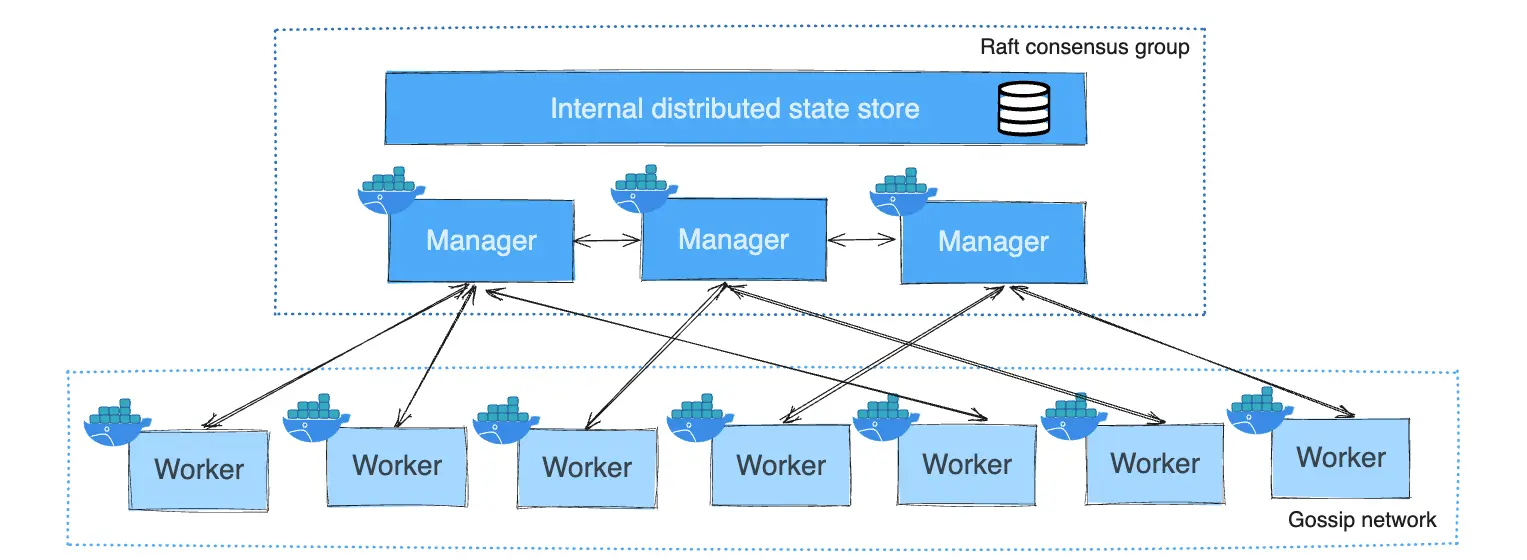
\includegraphics[width=0.7\linewidth]{raft-consensus.png}
    \caption{Nodi in Docker Swarm \cite{docker_manage_nodes}}
    \label{fig:placeholder}
\end{figure}

\newpage

\section{Conclusioni}
Il progetto ha portato alla realizzazione di un prototipo di orchestratore, che riesce a gestire un sistema distribuito e l'obiettivo di gestire i cicli di vita dei container è stato raggiunto.

Si è riuscito a replicare diverse delle funzionalità dell'architettura di riferimento, per dimostrarlo ecco un confronto delle operazioni consentite dalla CLI di Docker Swarm rispetto all'orchestratore proposto:
\begin{itemize}
    \item swarm init / swarm join, si è deciso di avere una infrastruttura statica tramite il deploy del cluster tramite docker compose l'orchestratore è subito pronto a gestire dei nodi worker su cui eseguire dei task. 
    \item service create, è possibile creare un servizio in base alle necessità dell'utente che può essere eseguito come task sul cluster.
    \item service scale / service rm, è possibile decidere di scalare il numero di repliche di un determinato servizio con la possibilità di azzerare quelle repliche.
    \item service ps, l'orchestratore permette di mostrare i task che stanno attualmente venendo eseguiti sui vari nodi.
    \item docker node ls / docker node ps, tramite le funzionalità introdotte dall'orchestratore è possibile visualizzare la topologia del cluster, il loro stato attuale e i loro task attivi. 
    \item docker node update, è permesso cambiare lo stato di un nodo per farlo passare in Drain così da svuotare i suoi task e passarli su altri nodi, impedendo al nodo di ricevere nuovi task. Così come è possibile renderlo nuovamente attivo per ricevere i task.
\end{itemize}

Il sistema soddisfa anche alcuni dei requisiti di un'architettura distribuita attraverso queste caratteristiche:
\begin{itemize}
    \item Load Balancing, caratteristica garantita dalle politiche di scheduling least loadead dell'orchestratore che permette di distribuire i task tra i nodi in maniera equa in base al nodo con meno task attivi. Oltre allo scheduling most loaded per la rimozione di task sui nodi che hanno più task attivi al momento per bilanciare il sistema in modo efficace senza sovraccaricare i singoli nodi.
    \item Fault Tolerance, grazie all'uso di un heartbeat per controllare lo stato attuale di nodi è stato possibile riconoscere i fallimenti e usare una meccanica active-active failover per i nodi così da rispondere correttamente ai fallimenti tramite la esecuzione dei task su altri nodi.
    \item Garbage Collection, è stato possibile riconoscere task spente sui nodi così da prevenire l'accumulo di oggetti non utilizzati ed evitando il degrado delle prestazioni sui nodi worker.
\end{itemize}

Nonostante le semplificazioni adottate rispetto a Docker Swarm, il prototipo di orchestratore ha dimostrato di riuscire a gestire i cicli di vita dei container attivi sui nodi e riesce ad implementare alcune caratteristiche fondamentali dei sistemi distribuiti.

\newpage
\addcontentsline{toc}{section}{Bibliografia}

\begin{thebibliography}{99}

\bibitem{silberschatz2014}
A. Silberschatz, P. B. Galvin, e G. Gagne, \textit{Sistemi operativi. Concetti fondamentali}, 9a ed., Milano: Pearson, marzo 2014.

\bibitem{tanenbaum_distributed_systems_4}
M. Van Steen e A. S. Tanenbaum,
\textit{Distributed Systems}, 4ª ed.,
Maarten van Steen, 2023.


\bibitem{ibm_orchestratore}
S. Susnjara e I. Smalley,
\textit{What Is Container Orchestration?},
IBM Think, 22 ottobre 2024.
[Online]. Disponibile: \url{https://www.ibm.com/think/topics/container-orchestration}.

\bibitem{oracle_docker}
Oracle Cloud Native, 8 dicembre 2025.
[Online]. Disponibile: \url{https://www.oracle.com/se/cloud/cloud-native/container-registry/what-is-docker/}.

\bibitem{docker_documentazione_security}
Docker Inc.,
\textit{Docker Engine Security: Linux Namespaces}, Docker Documentation.
[Online]. Disponibile: \url{https://docs.docker.com/engine/security/}.

\bibitem{man_namespaces}
Linux Man Pages,
\textit{namespaces(7) — overview of Linux namespaces}, Linux Programmer's Manual.
[Online]. Disponibile: \url{https://man7.org/linux/man-pages/man7/namespaces.7.html}.

\bibitem{man_cgroups}
Linux Man Pages,
\textit{cgroups(7) — overview of Linux control groups}, Linux Programmer's Manual, 2026.
[Online]. Disponibile: \url{https://man7.org/linux/man-pages/man7/cgroups.7.html}.

\bibitem{dockercon2023_dind}
Docker Inc.,
\textit{Docker-in-Docker and Containerized CI Workflows}, DockerCon 2023 Resources.
[Online]. Disponibile: \url{https://www.docker.com/resources/docker-in-docker-containerized-ci-workflows-dockercon-2023/}.

\bibitem{petazzoni_dind}
J. Petazzoni,
\textit{Using Docker-in-Docker for your CI or testing environment? Think twice}, 2015.
[Online]. Disponibile: \url{https://jpetazzo.github.io/2015/09/03/do-not-use-docker-in-docker-for-ci/}.

\bibitem{docker_swarm}
Docker Inc.,
\textit{Swarm mode overview}, Docker Documentation, 2026.
[Online]. Disponibile: \url{https://docs.docker.com/engine/swarm/}.

\bibitem{docker_swarm_key_concepts}
Docker Inc.,
\textit{Swarm mode key concepts}, Docker Documentation, 2026.
[Online]. Disponibile: \url{https://docs.docker.com/engine/swarm/key-concepts/}.

\bibitem{immagine_servizi_swarm}
J. J. Smile,
\textit{Docker Swarm Architecture and Concepts}, DevOps Notes, 2021.
[Online]. Disponibile: \url{https://smilejj91.github.io/devops/Docker-swarm/}.

\bibitem{supportlobby_swarm}
ActiveLobby Team,
\textit{What is Docker Swarm}, ActiveLobby Blogs, 2020.
[Online]. Disponibile: \url{https://blog.supportlobby.com/what-is-docker-swarm/}.

\bibitem{docker_swarm_cli}
Docker Inc.,
\textit{Docker Swarm CLI Reference}, Docker Documentation, 2026.
[Online]. Disponibile: \url{https://docs.docker.com/reference/cli/docker/swarm/}.

\bibitem{docker_service_cli}
Docker Inc.,
\textit{Docker Service CLI Reference}, Docker Documentation, 2026.
[Online]. Disponibile: \url{https://docs.docker.com/reference/cli/docker/service/}.

\bibitem{docker_node_cli}
Docker Inc.,
\textit{Docker Node CLI Reference}, Docker Documentation, 2026.
[Online]. Disponibile: \url{https://docs.docker.com/reference/cli/docker/node/}.

\bibitem{docker_manage_nodes}
Docker Inc.,
\textit{Manage nodes in a swarm}, Docker Documentation, 2026.
[Online]. Disponibile: \url{https://docs.docker.com/engine/swarm/manage-nodes/}.

\bibitem{mathworks_fdir}
MathWorks,
\textit{What Is Fault Detection, Isolation, and Recovery (FDIR)?}, MathWorks Discovery Pages, 2026.
[Online]. Disponibile: \url{https://in.mathworks.com/discovery/fdir.html}.

\bibitem{docker_how_services_work}
Docker Inc.,
\textit{How Swarm services work}, Docker Documentation, 2026.
[Online]. Disponibile: \url{https://docs.docker.com/engine/swarm/how-swarm-mode-works/services/}.

\bibitem{docker_pruning}
Docker Inc.,
\textit{Prune unused Docker objects}, Docker Documentation, 2026.
[Online]. Disponibile: \url{https://docs.docker.com/engine/manage-resources/pruning/}.

\bibitem{docker-raft}
Docker Documentation, \textit{Raft consensus algorithm in Swarm mode}. 
Disponibile online: \url{https://docs.docker.com/engine/swarm/raft/}
\end{thebibliography}
\end{document}
